%% !TEX root = ../ThesisManuscript_SJ.tex
%%
%%
%%	INTRODUCTION
%%_______________________________________________
\chapter{General introduction} 
\label{Introduction} 
\markboth{GENERAL INTRODUCTION}{}

\addtocontents{lof}{\protect\contentsline{chapter}{\protect\numberline{}Chapter \thechapter \medskip}{}{}}
\addtocontents{lot}{\protect\contentsline{chapter}{\protect\numberline{}Chapter \thechapter \medskip}{}{}}

\section{The prevention of infectious diseases}
\label{Intro:Prevention}

The prevention of infectious diseases has greatly improved, not only as a result of the development of safe, highly-effective preventive %and therapeutical 
methods, but also thanks to regional and global public health programs aiming for infectious diseases' elimination. During the last decade, the World Health Organization (WHO) developed the Global Vaccine Action Plan (GVAP) 2011--2020, aiming to ensure individuals to live free from vaccine-preventable diseases~\cite[]{GVAP_Review2020}. As a result, vaccine coverage among children and vaccine development have shown a remarkable progress, but many of the objectives remained unmet~\cite[]{GVAP_Review2020}. Disease-specific programs were also developed to fight infectious diseases' epidemics. For instance, the Global Measles%\footnote{Highly contagious viral infection, characterized by a rash, that can sometimes cause severe consequences, including death~\cite[]{CDC_PinkBook}.} 
and Rubella Strategic Plan 2012--2020~\cite[]{WHO_MR2012}, and the Fast Track to end AIDS epidemic~\cite[]{UNAIDS_EndAIDS2011}. 

%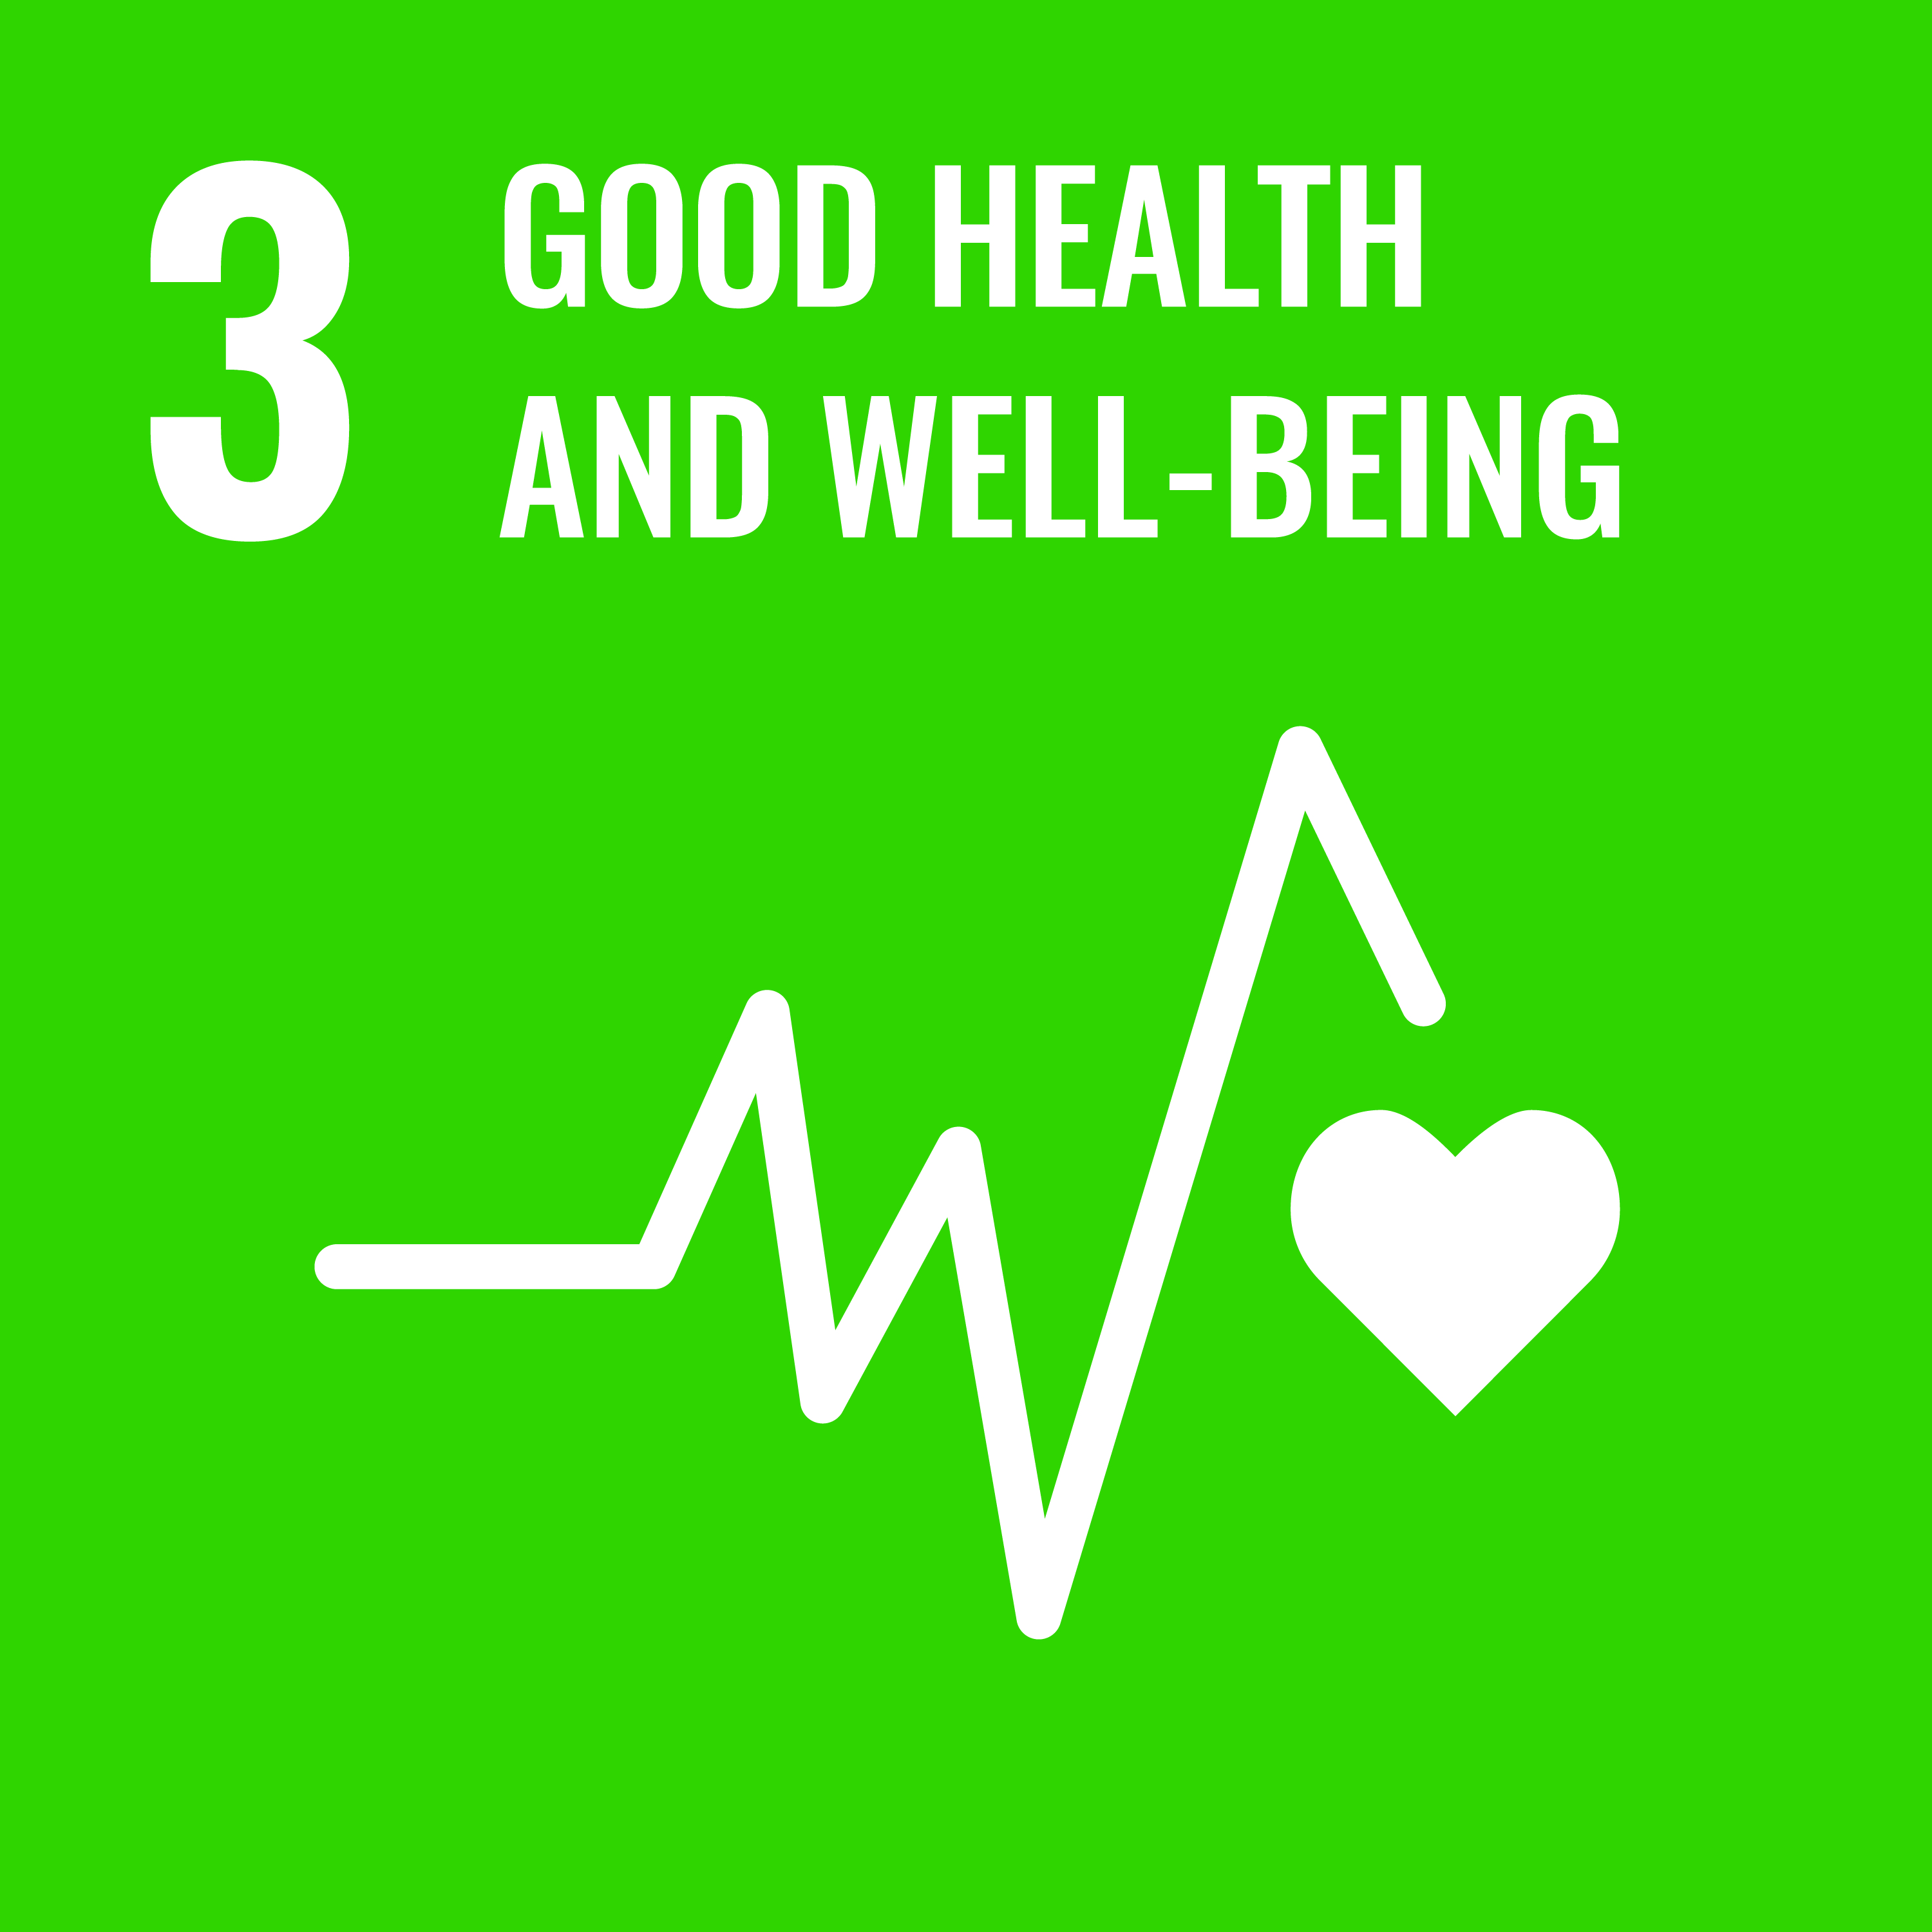
\includegraphics[width=2cm]{Figures/Intro/Goal3_SDG} 

Nowadays, disease-prevention interventions are included in the WHO's 17 Sustainable Development Goals; specifically, in the 3rd goal: ``To ensure healthy lives and promote well-being for all at all ages''~\cite[]{SDG_Goal3}. The objectives concerning communicable diseases include to end, by 2030, the epidemics of AIDS, tuberculosis, malaria and neglected tropical diseases, as well as to end preventable deaths of newborns and children under 5 years of age~\cite[]{SDG_Goal3}. The currently ongoing Immunization Agenda 2030, the successor of the GVAP 2011--2020, continues to place immunization in the core of national strategies for primary health care and universal health coverage~ \cite[]{WHO_IA2030}. In parallel, a global program to end sexually transmitted diseases by 2030 is ongoing, aiming, for instance, to the elimination of cervical cancer through vaccination interventions against human papillomavirus~\cite[]{WHO_STIs}. The Fast Track initiative to end the AIDS
%\footnote{Disease caused by the HIV virus, which targets the immune system, reducing the defense against other infections~\cite[]{WHO_Factsheet_HIV}.} 
epidemic is still ongoing, setting more ambitious and inclusive targets~\cite[]{UNAIDS_EndAIDS2030}. 

Global preventive interventions have successfully impacted epidemics. Immunization alone can now prevent more than 20 life-threatening diseases~\cite[]{WHO_IA2030}. Between 2000 and 2018, vaccination against measles prevented an estimated 23 million deaths~\cite[]{WHO_Factsheet_Measles}; during the same period, the number of new HIV infections fell by 39\%, thanks to preventive interventions~\cite[]{WHO_Factsheet_HIV}. The number of cases of poliomyelitis %
%\footnote{Viral infection of the nervous system causing lifelong paralysis~\cite[]{CDC_PinkBook}.} 
(commonly known as polio) have decreased from an estimated 350~000 cases in 1988, to 33 reported cases in 2018~\cite[]{WHO_Factsheet_Polio}. Meningococcal meningitis' %
%\footnote{Bacterial infection causing the inflammation of the membranes surrounding the brain. Complications may include disabilities and sepsis~\cite[]{CDC_PinkBook}.}%
incidence has decreased by 58\% in a relatively short period of time~\cite[]{WHO_Factsheet_Meningitis}. Mass immunization programs achieved the eradication of smallpox in 1980%
\footnote{During the pre-vaccination era, the mortality rate due to smallpox infection were about 30\%~\cite[]{CDC_Smallpox2001}.}
~\cite[]{CDC_Smallpox2001}. Preventive interventions have decreased the overall number of new infections worldwide~\cite[]{CDC_10achievements} and placed some communicable diseases (such as measles and poliomyelitis) in the path towards elimination~\cite[]{CDC_10achievements}. 


\subsection{Declaring epidemic elimination}  \label{Intro:EpiElim}

Global (respectively, regional) epidemic elimination refers to the end of an epidemic as a public health concern, through a high or a complete reduction of the infectious disease transmission worldwide (respectively, in the region), during a period of active surveillance~\cite[]{Porta2014,Nishiura2016}. Disease elimination does not imply the complete termination of disease transmission, nor the elimination of the infectious agent, as opposed to disease \emph{eradication}~\cite[]{Porta2014}. 

Therefore, global programs aiming to disease elimination set specific targets to be met in a certain amount of time and thus, declaring disease elimination may depend on the specific infectious disease and the context. %
Table~\ref{table:InfDisElim} shows some disease-specific targets, currently included in WHO programs aiming regional and/or global elimination.
The classical approach of the WHO to declare the end of an epidemic is to observe a significant period of time (for instance, twice as long as the empirical maximum of the incubation period) passed after the last reported case~\cite[]{Nishiura2016}. However, the case-free period approach to determine disease elimination may depend highly on the sample size, be inappropriate for diseases with high proportions of asymptomatic cases~\cite[]{Nishiura2016}, and depend greatly on prevention coverage~\cite[]{Eichner1996}. Other, rather heuristic ways to determine the end of an epidemic may also be used, depending on specific settings. For instance, the declaration of the elimination of the Middle East respiratory syndrome (MERS) in Korea was made after the removal of movement restriction for the last quarantined case~\cite[]{Nishiura2016}.

These kind of difficulties may be overcome using mathematical models to estimate the end of an epidemic. For instance, modeling studies have found that asymptomatic cases of poliomyelitis infection may still occur with a probability lower than 1\%, after 5 years of having no symptomatic cases within a 200\,000 population~\cite[]{Eichner1996}. In addition, mathematical modeling may provide estimates of unobserved variables and parameters, as well as identify the criteria to be met to end an epidemic; thus being useful to set public health targets for epidemic elimination.

\begin{landscape}
\captionsetup{width=1.3\textwidth}
\begin{table}[H]
	\centering
	\small
	\begin{tabular}{llll}
	\toprule
	\bf Infectious disease & \bf  Main targets & \bf Target year &\bf Ref.\\
	\toprule
	\bf HIV 		& $\bullet$ 90\% reduction of transmissions, compared to 2010 & 2030 & \cite[]{UNAIDS_EndAIDS2030}\\ 
				& $\bullet$ 95\% of infected people to know their HIV status & &\\
				& $\bullet$ 95\% of diagnosed people to be on treatment & &\\
				& $\bullet$ 95\% of people on treatment to have suppressed viral load & &\\ \midrule
	\bf Measles 	& $\bullet$ Absence of cases for at least 3 years & 2020\textsuperscript{a,b}  &  \cite[]{WHO_GVAP2018} \\
				& $\bullet$ Regional high vaccination coverage & &\\\midrule
	\bf Poliomyelitis & $\bullet$ Absence of cases for at least 3 years &&\cite[]{Eichner1996}\\
				& $\bullet$ No circulation of wild strain & &\\ \midrule
	\bf Rubella 	& $\bullet$ Regional 95\% reduction in the number of cases & 2020\textsuperscript{b}  & \cite[]{WHO_GVAP2018}\\
				& $\bullet$ Absence of cases for at least 3 years  & &\\
				& $\bullet$ Regional high vaccination coverage & &\\ \midrule
%	\bf Viral hepatitis & Reduce new cases of chronic viral hepatitis B infections by 95\% & 2030 & \cite[]{UN_IA2030}\\
	\bf Yellow fever & $\bullet$ Reduce outbreaks to zero & 2026 & \cite[]{WHO_IA2030}\\
	\bottomrule
\end{tabular}
	\caption[Targets of some recent, global programs aiming to end infectious diseases]{%
	\textbf{Targets of some recent, global programs aiming to end infectious diseases}\\
	Some recently disease-specific targets set within the WHO programs aiming to end epidemics. \\
	{\rule{5.5cm}{0.5pt}\\
	\footnotesize
	\textsuperscript{a} The American region was certified as having eliminated measles in 2016, after high vaccination coverage efforts, but lost its certification in 2018, after observing several outbreaks. Measles is currently endemic in all regions~\cite[]{GVAP_Review2020}.\\
	\textsuperscript{b} Unmet targets.}
	}
\label{table:InfDisElim}
\end{table}
\end{landscape}

%\subsubsection*{The prevention of infectious diseases: a multi-disciplinary, multi-level challenge}
%
%\rev{The success of public health programs aiming to epidemic elimination relies on many ... at many different levels. From the development of effective preventive and therapeutic tools, to the logistics ensuring availability and facilitating access. International or regional epidemiological targets require joint research and collaboration at the same scale. At the same time, the program implementations' adaptation to the local infrastructure and socio-cultural contexts is essential. }
%
%Ressource allocation and research funding. Public health authorities deploy prevention programs, ensuring constant feedback from the public, gathering surveillance data and sharing it with the public. 
%
%Prevention program also on the public participation, and thus, depend on the individual acceptance and adoption of the interventions. Hence, the role of the media and communication departments becomes important too, for an informed decision-making needs clear, accurate, opportune information. 
%
%Here, we focus in the role of the individual-level decision-making, facing epidemic threat in a context where efficient preventive and therapeutic methods are available, from the epidemiological and mathematical modeling perspective.

\section{The prevention versus treatment dilemma}
\label{Intro:Dilemma}

``An ounce of prevention is worth a pound of cure'', goes the popular saying. Yet, the individuals' preference for prevention over treatment may not be guaranteed. Some studies have indeed found a preference for prevention~\cite[]{Bosworth2010,Mortimer2008}, while others have found a preference for treatment~\cite[]{Corso2002,Schwappach2002} or not a significant preference~\cite[]{Ubel1998}. Preference has also been found to vary widely according, for instance, to age and health state~\cite[]{Luyten2015} and to the perceived urgency of the intervention~\cite[]{Meertens2013}. 

In high-income settings, individuals may face some difficulties and discomfort when adopting new behaviors and thus, individuals' attitudes towards prevention may differ from the public health authorities' recommendations. Therefore, when facing the risk of an epidemic, in a context where efficient treatment is available, individuals who find themselves at risk of infection may engage in a \textit{prevention versus treatment dilemma}, and make the decision between adopting prevention or not, and be treated in case of infection. 

The adoption of prevention thus depends mainly on the individuals' perception of its benefits and inconveniences versus those of treatment, as well as their perception on their own risk of infection. Public health authorities and healthcare providers may play an essential role shaping these perceptions. For instance, by sharing information about epidemics and disease burden, as well as providing information on the available preventive and therapeutic tools, and increasing their availability and access.%~\cite[]{Larson2016,Coleman2017}.

\textit{Voluntary prevention} is defined as the preventive methods adopted voluntarily by individuals to avoid infection. That is, by willingly following the recommendations of public health authorities' --- in contrast to mandatory\footnote{Required by law or community rules.} prevention. To evaluate the impact of voluntary prevention on the epidemic dynamics, it is thus essential to account for individuals' resolution of the prevention versus treatment dilemma. %In particular, mathematical models can be used to study disease transmission accounting for individual behavior, and to identify the conditions to be met by public health interventions aiming epidemic elimination.
%
Here, we focus in the role of the individual-level decision-making, facing epidemic threat in a context where efficient preventive and therapeutic methods are available, from the epidemiological and mathematical modeling perspective.

\section{Mathematical and behavioral epidemiology of infectious diseases}
\label{Intro:BehavEpi} 

Mathematical modeling of infectious diseases was used to assist public health decision-making for the first time in 1760\footnote{The paper was first presented at the Royal Academy of Sciences in Paris in 1760 and then published in 1766.}, when Daniel Bernoulli (1700--1782) studied smallpox and recommended universal inoculation to prevent smallpox-related mortality: ``...it has been noticed that, on the one hand, the more natural smallpox spreads, the more dangerous it is; and, on the other, that inoculation carried out at the height of an epidemic is not by any means as reliable as if it were done quite outside any epidemic''~\cite[]{Bernoulli1766,Blower2004}. Bernoulli's recommendation was based on his estimation of the number of lives saved by universal inoculation against smallpox~\cite[]{Blower2004}. The model proposed by Bernoulli consisted in analyzing surveillance data consisting in the yearly number of individuals who had been infected, the number of deaths due to smallpox infection, etc. Then, he compared the number of smallpox deaths before and after the adoption of inoculation amid the population~\cite[]{Blower2004,Dietz2002}. In his paper, Bernoulli also acknowledged that individuals could be interested in being inoculated because of the benefits it offered at the individual level (such as avoiding lethal infection), versus those offered at the population level (such as increasing the average life expectancy).

Since the 18th century, different kinds of models have been developed to describe epidemic dynamics~\cite[]{Brauer2017}. 
% Ejemplos de modelos?
Mathematical models are useful to understand the transmission mechanisms behind surveillance data, to estimate the values of parameters that cannot be directly measured, to predict disease epidemiology and to select intervention designs aiming to control the epidemic and or the disease burden~\cite[]{Valleron2000}. Mathematical epidemiology has thus become a powerful tool for public health decision-making and epidemic control~\cite[]{Valleron2000}. 

Behavioral epidemiology is a relatively recent branch of mathematical epidemiology that studies the interplay between the human behavior and the course of an epidemic~\cite[]{Manfredi2013,Verelst2016,Wang2016}. Behavioral epidemiology accounts for the role of human behavior as a key component of epidemic spread and the implementation of public health policies. For instance, by taking into account the changes in individual behavior as a response to epidemic dynamics and epidemic threats, as well as the individual attitudes towards the available preventive methods.

From the modeling perspective, the issue of voluntary prevention and its impact on the epidemic has been addressed using hybrid models that combine mathematical models describing the disease transmission at the population level, with models describing the individual's adoption of preventive methods to avoid being infected~\cite[]{Verelst2016}. The infectious disease transmission has been modeled using mostly deterministic compartimental models\footnote{As opposed to stochastic models (that can also be compartmental), which can be particularly useful to model disease transmission among small populations.}  and individual-based models (which allow to consider some stochasticity). The adoption of prevention has been modeled, for instance, by a change in the individual's susceptibility to the infection (such as being immunized), a change in the model parameters (such as reducing disease transmissibility) or a change in the contact structure (such as reducing the number of contacts with other individuals, which is known as \textit{social distancing}); see~\cite[]{Verelst2016}. Traditionally, hybrid models studying social distancing use the individual-based models for the disease transmission, while those studying vaccination use compartimental models~\cite[]{Verelst2016}.

In behavioral epidemiology, individuals are assumed to translate the information about epidemic dynamics into behavioral changes; i.e., acknowledging their risk of infection and making informed decisions. The information about the epidemic has been previously modeled as epidemiological indicators ---assumed to be provided to individuals by public health authorities---, as well as subjective perceptions and/or rumors~\cite[]{Verelst2016}. The interaction between the epidemiological information and the change in behavior has been modeled, for instance, as a threshold that triggers the prevention adoption, or as a dynamic parameter which affects and is affected by prevention adoption~\cite[]{Verelst2016}. Some models have used the risk of infection perceived by individuals to explicitly address the prevention versus treatment dilemma (see~\secref{Intro:DecisionModel}).

%Only a few hybrid models validate their model using available data~\cite[]{Verelst2016}.
 
							
\subsection{Modeling disease transmission using deterministic compartmental models}

Deterministic compartimental models have been widely used to model disease transmission among large populations~\cite[]{Brauer2017}. These models are defined by a system of ordinary differential equations (ODE), whose state variables represent the number or proportion of individuals in each compartment, and whose parameters represent the rates of transition from one compartment to another~\cite[]{Hethcote2000}; for instance, from susceptible to infected, then to infectious or contagious, to recovered, dead, and so on. The transition of individuals from being susceptible to being infected, is often modeled by the \textit{force of infection} (or infection rate), which depends on the disease transmission mechanisms, such as the contacts between uninfected and infectious individuals, and their probabilities to occur. 

Classical compartmental models are usually named by acronyms obtained from merging the initials of the compartment variables. For instance, a model considering only susceptible, infected and recovered individuals is called an $SIR$ model. The Bernoulli's paper mentioned in the previous section can be represented by an $SI$ model~\cite[]{Dietz2002}. 
%
Figure~\ref{fig:Intro_MSIR} depicts a paradigm example of a classical compartmental model accounting for newborns immunization. Susceptible individuals ($S$) get infected ($I$) and then, recover ($R$). Considering an imperfect preventive method allows to model individuals getting infected despite having been previously immunized\footnote{On the contrary, in the case where perfect immunity is considered, immunized individuals are directly removed from the population --- to the Recovered compartment.}. To keep track of immunized individuals, the immunity induced by a preventive method is included in the model by adding, for instance, a compartment representing the proportion of newborns who are immunized ($M$). The classical $SIR$ thus becomes a $MSIR$ model.

\begin{figure}[H]
	\centering	
	%% DRAFT
%	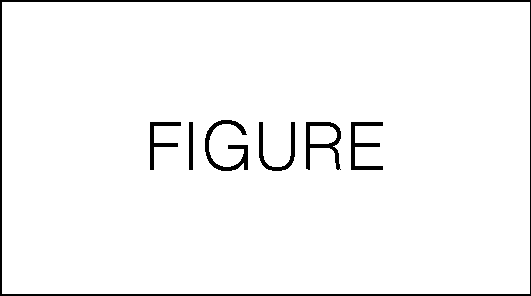
\includegraphics[width=0.6\textwidth]{DRAFT_FigsAndDocs/FIG}
	%%
	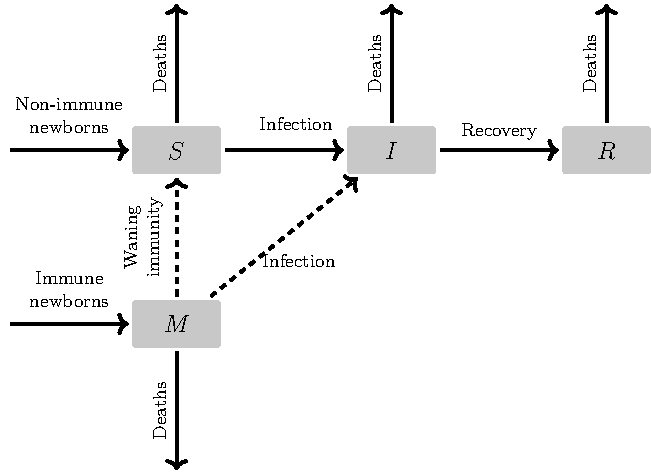
\includegraphics[width=0.6\textwidth]{Figures/Intro/TikZ_MSIR/MSIR_FlowDiagram}
	\caption[ Conceptual compartimental model with prevention]{%
		{\bf Conceptual compartimental model with prevention}\\
	Flow diagram of a classical \textit{SIR}-type compartimental model, describing the transmission of an infectious agent  and disease progression, among a population by modeling individuals' transitions through different states, during their lifetimes. Some of the newborns may be immunized ($M$) against the infectious disease or not. Susceptible ($S$) individuals get infected ($I$) and then recover ($R$). Depending on the level of protection offered by the preventive method, immunized individuals may get infected, nevertheless, and/or immunity may wane with time (dashed arrows). Individuals leave the population by dying.}
	\label{fig:Intro_MSIR}
\end{figure}
 
More complex compartmental models can include population stratification by disease progression (e.g., acute infection, chronic or asymptomatic period), kind of case resolutions (e.g., removal, recovery, death), demographics (e.g., age, sex), exposure to the disease (e.g., risk of infection, number of contacts), use of preventive and/or therapeutic tools, etc.~\cite[]{Hethcote2000}. 


%\subsection{Using the basic and the effective reproduction numbers to determine the impact of preventive methods}
\subsection{The basic and the effective reproduction numbers}
\label{Intro:ReproductionNumbers}

The \textit{basic reproduction number}, noted $R_0$, is defined as the expected number of secondary cases produced by a single infectious individual, during the entire infectious period, in a fully susceptible population~\cite[]{Anderson1991,Heesterbeek2002}. The \textit{effective reproduction number} ---also called the replacement number--- is defined as the expected number of secondary cases produced by an infectious individual, at a given time or in a given context; for instance, once the population is subject to interventions such as prevention and treatment~\cite[]{Ridenhour2018,VanDenDriessche2008,VanDenDriessche2002,Hethcote2000}. In other words, the effective reproduction number represents the number of secondary infections occurring at a time $t$, whereas the basic reproduction number represents a theoretical number of secondary cases occurring in the absence of previous infections and interventions, and thus, independent of time. 

The basic and the effective reproduction numbers reflect epidemic severity, and thus are useful to study the impact of preventive methods on epidemic dynamics: a large basic reproduction number corresponds to a fast epidemic spread throughout the population; a decrease in the effective reproduction number reflects epidemic mitigation. 

The basic and the effective reproduction numbers can be estimated using mathematical models~\cite[]{Ridenhour2018,Guerra2017}. In particular, they can be computed from deterministic compartmental models, and thus be expressed as functions of the ODE system parameters~\cite[]{Heffernan2005,VanDenDriessche2002,VanDenDriessche2008}. Notably, there exists a relation between the reproduction numbers and the behavior of the ODE system at the equilibrium~\cite[]{VanDenDriessche2002}. ODE systems defining classical compartimental models for disease transmission, similar to the model depicted in~\figref{fig:Intro_MSIR}, often have two equilibria: a disease-free state (DFS), where there are no new infections, and an endemic state (ES), where the epidemic persists~\cite[]{Hethcote2000,VanDenDriessche2002}. A reproduction number is a threshold parameter for the ODE system equilibria: there is a transcritical bifurcation (that is, an exchange in the stability of the equilibria) for the ODE system when the reproduction number equals to 1. When the reproduction number is lower than 1, the ODE system reaches the DFS and thus the epidemic is eliminated in the long run; otherwise, the ODE system will reach the ES~\cite[]{Hethcote2000,VanDenDriessche2002}. See~\figref{fig:Intro_Bifurcation} for a conceptual visualization of the transcritical bifurcation.

\begin{figure}[H]
	\centering	
	%% DRAFT
%	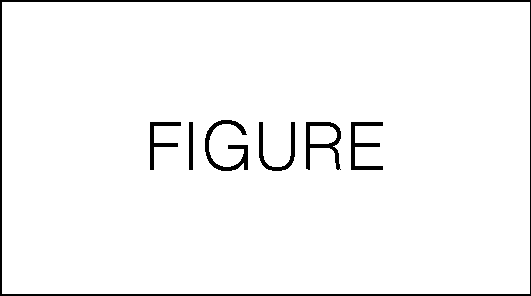
\includegraphics[width=0.7\textwidth]{DRAFT_FigsAndDocs/FIG}
	%%
	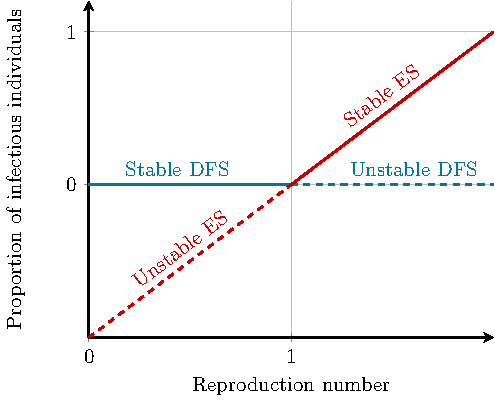
\includegraphics{Figures/Intro/TikZ_Bifurcation/TranscriticalBifurcation}
	\caption[ Conceptual visualization of the bifurcation diagram for an ODE system]{%
		{\bf Conceptual visualization of the bifurcation diagram for an ODE system}\\
	Classical ODE systems describing disease transmission usually have two equilibria: the disease-free state (DFS, depicted in blue), where there are no new infections, and the endemic state (ES, depicted in red), where the epidemic persists. A change in stability of the equilibria occurs when the reproduction number equals to 1 (depicted by the transition from a solid to a dashed line). Note that negative populations (red, dashed line), while correspond to some the solutions of the ODE system mathematically, have no biological interpretation.}
	\label{fig:Intro_Bifurcation}
\end{figure}

\subsubsection*{Herd immunity: a public health target} \label{sec:Intro_HerdImmunity}

Prevention-induced \textit{herd} or \textit{community immunity} refers to the situation in which susceptible individuals are indirectly protected against infection, due to a sufficiently large proportion of the population adopting the preventive method against the pathogen. As a result, disease transmission is greatly reduced and the population is said to be immune as a group; the epidemic is expected to be eliminated in the long run (i.e., the DFS is reached)~\cite[]{Porta2014,Fine2011,CDC_Epidemiology,Anderson1992}.

From the modeling perspective, the proportion of individuals required to adopt prevention, for the community to reach herd immunity, is obtained from the level of prevention coverage (i.e., the proportion of the population that has adopted the preventive method) required for the effective reproduction number to be below 1. The larger the basic reproduction number, the larger the prevention coverage required to eliminate the epidemic. 

Public health authorities usually set the target for prevention interventions depending on the prevention coverage threshold that gives herd immunity. However, as discussed in~\secref{Intro:Dilemma}, different public sentiments and strategies towards the prevention versus treatment may yield a sub-optimal prevention coverage (i.e., lower than the prevention coverage threshold). 
Hence, it key for public health authorities to know whether voluntary prevention coverage can deliver the level needed for herd immunity. 


\subsection{Modeling the decision-making about prevention adoption}
\label{Intro:DecisionModel}

Among the mathematical models accounting for behavioral change, game-theoretic approaches have been used to address the individual's decision-making facing the prevention versus treatment dilemma~\cite[]{Bauch2013,Verelst2016,Wang2016,Chang2020}. Game theory is a mathematical discipline that allows to model rational individual's decision-making and selection of strategies through the assessment of risk and payoff. The individuals' decisions are modeled by finding the equilibrium set of strategies; that is, the strategies that individuals benefit the most from, in the long run~\cite[]{Manfredi2013}. In particular, the prevention versus treatment dilemma may be modeled by the comparison of the payoff expected for adopting the strategy of using prevention, with that of adopting the strategy of being treated in the case of infection.

%\rev{An early paper studying public health policies on pertussis vaccination, taking into account the individual decision-making about getting vaccinated, found that the most beneficial strategy for individuals may differ from the optimal strategy for the population (which minimizes the total morbidity faced by the population). The paper discusses how the individual-level strategy }

\rev{Minimization of perceived cost}

\begin{equation}
	\text{Total cost} = 
\end{equation}


Most studies using game-theoretic models for individual decision-making have used deterministic, compartimental models to describe the epidemic dynamics at the population level~\cite[]{Bauch2003,Bauch2004,Breban2006,DOnofrio2007,Vardavas2007,Galvani2007,Breban2011,Liu2012}. These hybrid models have been used to address, for instance, vaccination facing a biochemical attack~\cite[]{Bauch2003}, voluntary vaccination during a public scare of vaccination against childhood infectious disease~\cite[]{Bauch2004} and recurrent decision-making on preventing seasonal infections such as influenza~\cite[]{Breban2006,Galvani2007}. The risk of infection perceived by individuals has been defined, for instance, by a free parameter taking different values~\cite[]{Bauch2004}, by epidemiological indicators reflecting the current epidemiological situation~\cite[]{Bauch2003,DOnofrio2007,Breban2011,Liu2012} or considering the past experience of individuals facing the epidemic~\cite[]{Breban2006,Vardavas2007,DOnofrio2007}. Prevention has been considered to offer perfect immunity~\cite[]{Bauch2003,Bauch2004,DOnofrio2007} or short-term immunity, thus requiring recurrent decision-making~\cite[]{Breban2006}. 

These modeling studies have concluded that the level of prevention coverage achieved through selfish individual-level decisions  (i.e., decisions motivated by the individual's own interest) may differ from the level of prevention coverage needed to achieve herd immunity~\cite[]{Bauch2003,Bauch2004,Breban2006,Galvani2007,Breban2011}, unless incentives are offered~\cite[]{Vardavas2007,Liu2012}. % Others have found that stable oscillations may appear if individuals consider only past states of the epidemic, ignoring the current state~\cite[]{DOnofrio2007}. 
However, as discussed in \secref{Intro:Dilemma}, mass vaccination has resulted in epidemic elimination ---globally, regionally or at least temporarily ---, owing to vaccination campaigns facilitating vaccine adoption on nation-wide scales. Therefore, the impact of voluntary prevention on epidemic dynamics, and whether it can eliminate epidemics or not, remains to be studied.

\section{General objectives of my doctoral research}
\label{Intro:Objectives} 

The main objective of my doctoral research project was to build mathematical models for infectious disease transmission at the population-level, accounting for the individual-level decision-making on whether or not to adopt available preventive methods to avoid the infection, in a context where effective treatment exists. We aimed to evaluate the impact of the voluntary adoption of prevention on the epidemic dynamics. In particular, our purpose was to determine whether and under what conditions could voluntary prevention avert epidemics.

Two applications were explored. The first part of my thesis focuses on voluntary vaccination against treatable childhood infectious diseases; see~\autoref{Vaccine}. This first project was designed for analytical results. The second part of my thesis focuses on the voluntary use of pre-exposure prophylaxis by men who have sex with men and who are at high risk of infection, in the current context of the HIV epidemic, where highly effective antiretroviral therapies are available; see~\autoref{PrEP}. Due to the complexity of the HIV transmission model, the model was studied using numerical simulations.



\section{General description of our methods}

%\subsection{Conceptual framework}
%\label{Intro:Framework} 
%
%We study the interplay between individual behavior and infectious diseases' epidemic dynamics, in the context where effective treatment and imperfect preventive methods are available. We consider the adoption of prevention to be voluntary (that is, it is not a product of mandatory health policies), whereas treatment is assumed to be immediately adopted after diagnosis. That is, we do not study the individual's decision-making regarding the adoption of treatment. 
%
%Four hypotheses are key to this research project:
%
%\begin{enumerate}[label= \bf \roman*)]
%\item \textbf{Individuals' decision maximizes their own benefit.}
%
%When facing an ongoing epidemic, individuals address the prevention versus treatment dilemma by evaluating their risk of infection, its consequences, the availability of both preventive and therapeutic tools, and the related benefits and constraints. The individuals' decision-making is thus driven by weighing of the perceived pros and cons of prevention versus treatment, as well as their perception on the risk of infection. 
%
%Therefore, the individuals' decision on whether or not to adopt prevention to avoid the infection may be biased, yet closely related to the course of the epidemic. Indeed, the risk of infection depends on the disease's prevalence, which in turn depends on the efficacy and coverage of the preventive and therapeutic methods. Hence, each individual's decision is indirectly influenced by others' decisions, since the sum of all decisions determines the voluntary prevention coverage, which impacts the course of the epidemic.
%
%\item \textbf{Voluntary prevention coverage may differ from the estimated coverage for epidemic control, recommended by public health authorities.} 
%
%Since the individuals' perception of their risk of infection may be biased, the prevention coverage allowing to reach herd immunity may not be achieved. Therefore, increasing the acceptability of preventive methods becomes a key objective of public health authorities.

%\item \textbf{Prevention incentives are possible.} 
%
%Efforts may be done in order to increase the accessibility to preventive methods and to reduce the  prevention-related barriers perceived by individuals. For instance, public health programs and resource allocation may be directed to the implementation of measures encouraging prevention adoption.

%\item \textbf{Imperfect prevention methods may nevertheless avert epidemics.}
%
%Imperfect vaccines (lasting for a limited duration of time and taking only in a proportion of the population) have shown to be able to avert epidemics (e.g., measles~\cite[]{Sever2011}) and even to eradicate diseases (e.g., smallpox~\cite[]{CDC_Smallpox2001}), provided that the performance and coverage of preventive methods are sufficiently high.
%\end{enumerate}


\subsection{The mathematical model}
\label{Intro:Model} 

We coupled two components to build a mathematical model describing the interplay between epidemic dynamics and voluntary prevention: one for the infectious disease transmission at the population level and one for the decision-making on whether or not to use prevention, at the individual level. See~\figref{ModelDiagram} for a graphical depiction of our hybrid model. Details on the models specifically developed for each of the two applications are found in the following chapters. 

\begin{figure}[H]
	\centering	
	%% DRAFT
%	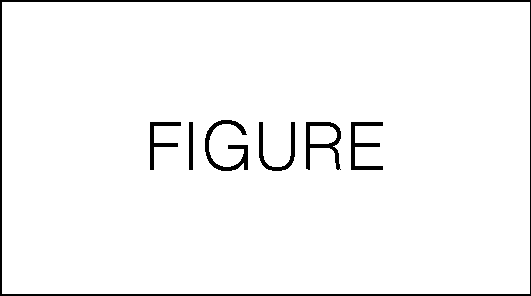
\includegraphics[width=0.8\textwidth]{DRAFT_FigsAndDocs/FIG}
	%%
	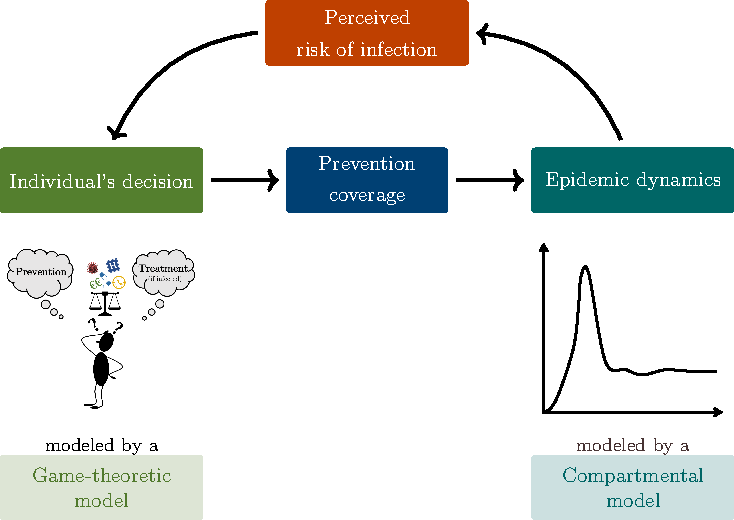
\includegraphics{Figures/Intro/TikZ_Model/ModelDiagram}
	\caption[Diagram of our hybrid model]{%
		{\bf Diagram of our hybrid model}\\
	When facing an ongoing epidemic, individuals address the prevention versus treatment dilemma by evaluating their risk of infection, its consequences, the availability of both preventive and therapeutic tools, and the related benefits and constraints. Therefore, the individuals' decision on whether or not to adopt a prevention method to avoid the infection may be biased, yet closely related to the course of the epidemic. Indeed, the risk of infection depends on the disease's prevalence, which in turn depends on the efficacy and coverage of the preventive and therapeutic methods. Hence, each individual's decision may be indirectly influenced by others' decisions, since the sum of all decisions determines the voluntary prevention coverage, which impacts the course of the epidemic.
	}
	\label{ModelDiagram}
\end{figure}

\subsubsection*{Modeling disease transmission at the population level}
To describe disease transmission within a population, we use a deterministic compartmental model, defined by a system of ODEs, which represents the individuals' infection and disease progression~\cite[]{Hethcote2000,Jacquez1988}. In addition, we consider a compartment representing individuals adopting prevention. We do not consider that prevention is 100\% effective and thus, individuals adopting prevention can nevertheless be infected. Therefore, our model explicitly accounts for two parameters regarding prevention: coverage and effectiveness.

We use the ODE system to compute epidemiological indicators such as the incidence rate, the disease prevalence, the number of diagnoses, etc., which can be expressed explicitly as functions of the prevention parameters. By computing these epidemiological indicators at the endemic state of the system\footnote{The existence of the endemic and the disease-free equilibria is studied in detail by~\citet{Hethcote2000} for the vaccination model and by~\citet{Jacquez1988} for the PrEP model.}, we observe the behavior of the epidemic in the long run, which will be useful for the decision-making component of the model (see below). 

We compute the effective reproduction number from the ODE system, following the methods developed by~\citet{VanDenDriessche2002}. We also express the effective reproduction number as a function of the prevention parameters, and we obtain the basic reproduction number by setting the prevention coverage equal to 0. In other words, the basic reproduction number reflects the epidemic's severity in the case where no prevention method is available. 

As mentioned in~\secref{Intro:ReproductionNumbers}, the effective reproduction number is used to study the impact of the preventive methods on the epidemic. We say that the epidemic is \textit{eliminated} or \textit{averted} by the prevention method if the effective reproduction number ---a function of the prevention parameters--- is below 1. If the effective reproduction number is inferior to the basic reproduction number, we say that the epidemic is \textit{controlled} by the preventive method, since a reduction in the effective reproduction number is reflected in a reduction in the epidemic's incidence.

We first use the effective reproduction number to determine the conditions under which disease elimination or disease persistence occur, in the long run, regardless of individual behavior. In particular, a threshold for the prevention coverage leading to epidemic elimination can be determined. Then, the introduction of the decision-making component allows to study whether and under what conditions this theoretical threshold for epidemic elimination could be reached voluntarily.

\subsubsection*{Modeling decision-making at the individual level}
To describe the individual's decision-making, we rely on a game-theoretical approach: a non-cooperative single-player game, where an individual is assumed to act in his own interest. We assume that individuals address the prevention versus treatment dilemma by evaluating their risk of infection and by weighing the benefits and inconveniences of the preventive method versus those of treatment, which include monetary and non monetary aspects, such as price, undesired secondary effects, difficulties in access, disease morbidity, etc. In a game-theoretic framework, these factors are known as {\it costs}. 

The fundamental tool for modeling decision-making is the individual's expected {\it utility}, which summarizes the individual's perception of the costs to pay for choosing one of two strategies before their risk of infection: to adopt prevention, or not (and be treated upon infection). Game theory postulates that rational decision-making can be mathematically modeled by maximizing the utility. In other words, the aim of using a game theoretic approach is to find the individuals' strategies that benefit them the most, in the long run. 

We formally define utility as a function of the endemic risk of infection and the {\it relative cost of prevention versus treatment}, perceived by individuals. We consider that individuals may acknowledge official estimations of the epidemiological indicators (which can be obtained, for instance, from the transmission model, and communicated to the public by health authorities, healthcare providers, scientific journalists, associations, etc.), but may also make their decision based on a misperception of their risk of infection. The relative cost remains a rather qualitative parameter that indicates how more beneficial is prevention perceived, over treatment.

The prevention coverage that maximizes the individual's expected utility gives the probability for an individual to voluntarily adopt prevention, as a function of the model parameters. Hence, we obtain the {\it voluntary prevention coverage}, the prevention coverage reached voluntarily by the individuals who perceive themselves as being at risk of infection. 
%
We study the voluntary prevention coverage in terms of the preventive method's parameters: effectiveness and the relative cost of prevention versus treatment. In particular, we look for the conditions for which the voluntary prevention coverage can yield epidemic control and/or elimination, through the reduction of the effective reproduction number.

